\documentclass[crop=false]{standalone}
\usepackage{standard}
\begin{document}
  \section{Einführung} % (fold)
  \label{sec:introduction}

    In der Physik werden wichtige Vorgänge der Natur oder technischer Prozesse durch partielle Differentialgleichungen (PDE) beschrieben.
    Gerade in der industriellen Forschung benötigt man Lösungen dieser Gleichungen, um neue Bauteile und Verfahren, die gewissen Bedingungen genügen müssen, zu konstruieren.
    Als Beispiel sei hier die Wärmeleitungsgleichung genannt, deren Lösung es ermöglicht die Temperaturverteilung eines solchen Bauteils zu bestimmen.
    Die Lösung weist auf die Schwächen und Stärken eines Bauteils hin, ohne dieses real konstruieren zu müssen.

    Die PDE praxisnaher Probleme sind jedoch meistens zu kompliziert, um sie analytisch zu lösen.
    Entweder es existiert nicht einmal eine geschlossene Lösung oder sie wäre viel zu kompliziert.
    Aus diesem Grund beschränkt man sich im Bereich der industriellen Forschung auf verschiedene numerische Verfahren zum Lösen dieser Gleichungen.
    Die erhaltenen Lösungen stellen zwar nur eine Approximation der eigentlichen Lösung dar, können diese jedoch meistens beliebig genau annähern.
    Typische Verfahren zum Lösen von PDE stellen die Finite-Differenzen-Methode, die Finite-Volumen-Methode und die Finite-Elemente-Methode dar.
    In Abbildung \ref{fig:intro} wird die numerische Simulation der Wellengleichungen anhand eines Beispiels demonstriert.

    \begin{figure}[h]
      \center
      \begin{subfigure}[b]{0.32\textwidth}
        \center
        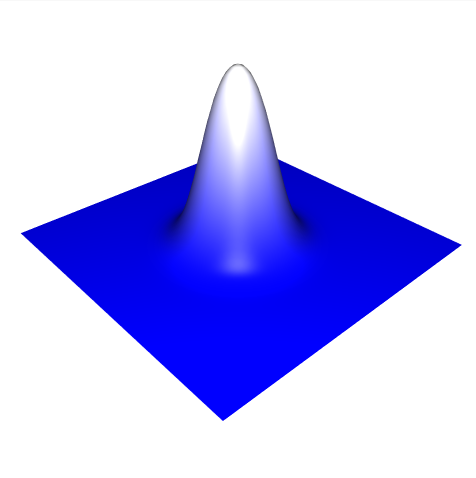
\includegraphics[trim={0 0 0 2.2cm}, clip, width=0.8\textwidth]{images/intro_01.png}
        \caption{}
      \end{subfigure}
      \begin{subfigure}[b]{0.32\textwidth}
        \center
        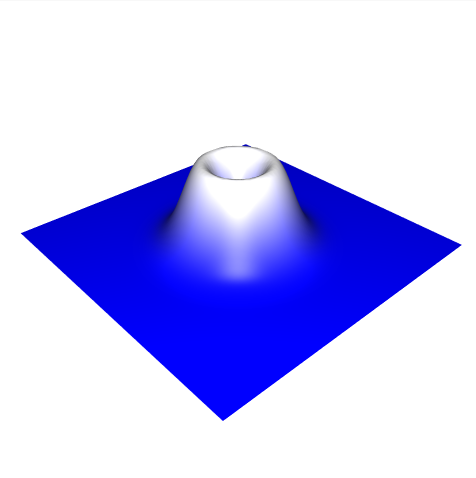
\includegraphics[trim={0 0 0 2.2cm}, clip, width=0.8\textwidth]{images/intro_02.png}
        \caption{}
      \end{subfigure}
      \begin{subfigure}[b]{0.32\textwidth}
        \center
        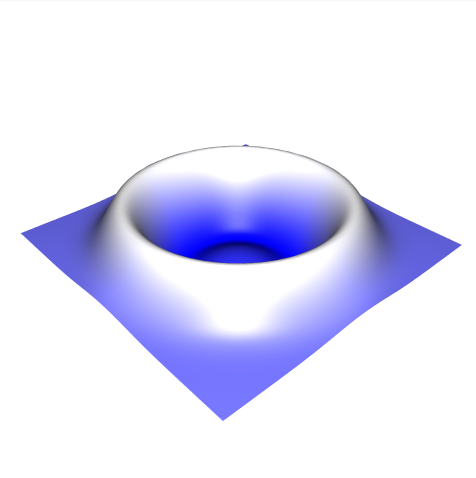
\includegraphics[trim={0 0 0 2.2cm}, clip, width=0.8\textwidth]{images/intro_03.png}
        \caption{}
      \end{subfigure}

      \begin{subfigure}[b]{0.32\textwidth}
        \center
        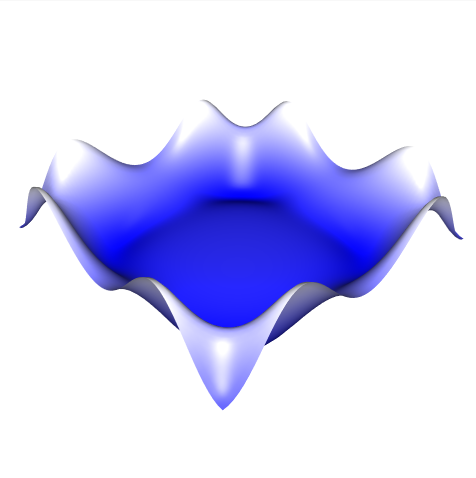
\includegraphics[trim={0 0 0 2.2cm}, clip, width=0.8\textwidth]{images/intro_04.png}
        \caption{}
      \end{subfigure}
      \begin{subfigure}[b]{0.32\textwidth}
        \center
        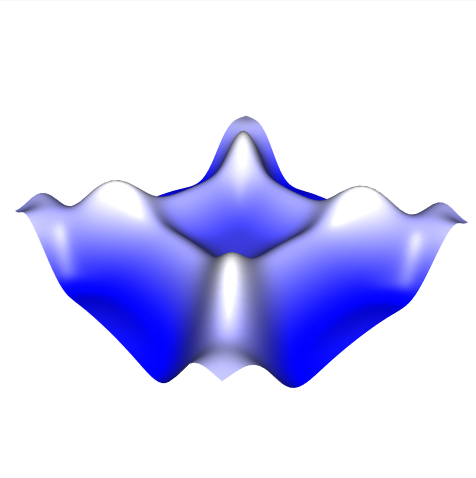
\includegraphics[trim={0 0 0 2.2cm}, clip, width=0.8\textwidth]{images/intro_05.png}
        \caption{}
      \end{subfigure}
      \begin{subfigure}[b]{0.32\textwidth}
        \center
        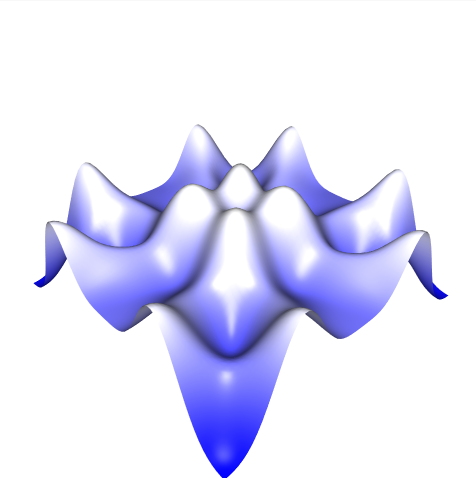
\includegraphics[trim={0 0 0 2.2cm}, clip, width=0.8\textwidth]{images/intro_06.png}
        \caption{}
      \end{subfigure}
      \caption[%
        Einfache Simulation der Wellengleichung%
      ]{%
        Die Abbildung zeigt die Evolution einer numerischen Lösung der Wellengleichung auf einem quadratischen zweidimensionalen Gebiet.
        Für die Berechnung wurde die hier implementierte FEM verwendet.%
      }
      \label{fig:intro}
    \end{figure}

    Die Finite-Elemente-Methode (FEM) stellt eines der allgemeinsten Verfahren zum numerischen Lösen von partiellen Differentialgleichungen dar.
    Aus diesem Grund ist deren Anwendung nicht auf ein konkretes physikalisches Gebiet beschränkt.
    Obwohl die FEM zunächst nur für die Strukturberechnung von Flugzeugflügeln in der Luft- und Raumfahrtindustrie verwendet wurde, findet sie heute in vielen Bereichen der Physik, wie zum Beispiel der Festigkeits- und Verformungsuntersuchung von Festkörpern, der gekoppelten Feldberechnung und bei Wettervorhersagen, ihre Anwendung.
    Aufgrund ihrer im Vergleich zu anderen Verfahren späten Entwicklung konnte die FEM computergerecht formuliert werden.
    Dennoch benötigt sie eine erhebliche Rechenleistung.

    Ein Vorteil der FEM besteht nun darin, dass sich viele der Berechnungen nur durch ihre Eingaben, aber nicht durch deren Algorithmen, unterscheiden.
    In einem FEM-Programm wird im Normalfall eine geringe Anzahl von Verzweigungen verwendet.
    Dieser Vorteil kann durch eine Implementierung auf der Grafikkarte ausgenutzt werden.
    Eine Grafikkarte arbeitet massiv parallel und ist somit in der Lage die Performance eines FEM-Programms um ein Vielfaches zu steigern.

  % section einführung (end)
\end{document}